%============================================================================%
% DOCUMENT DEFINITION
%============================================================================%
\documentclass[12pt,a4paper,english]{article}

%-----------------------------------------------------------------------------
% Page layout
%-----------------------------------------------------------------------------
% page outer frames (debug-only)
% \usepackage{showframe}

% define page styles using geometry
\usepackage[a4paper]{geometry}

% Margins
\geometry{top=2cm, bottom=2cm, left=2cm, right=2cm}

%-----------------------------------------------------------------------------
% Packages
%-----------------------------------------------------------------------------
% Math
\usepackage{amsmath}

% Extended implementation of the arrays and tabules
\usepackage{array}

% Languages
\usepackage[main=english, spanish]{babel}
\usepackage[spanish]{datetime2}
\usepackage{indentfirst}

% Enhances the quality of tables.
\usepackage{booktabs}

% To use the slash to cancel out stuff
\usepackage{cancel}

% Customise the captions in figures and table
\usepackage{caption}

% Enumeration
\usepackage{enumitem}

% fancy headers and footers
\usepackage{fancyhdr}
\usepackage{lastpage}

% Improves the interface for defining floating objects such as figures and tables.
\usepackage{float}
\restylefloat{table}
\usepackage{diagbox}

% The enhanced graphics package.
\usepackage{graphicx}
\graphicspath{{./}{./images}{./figures}{../shared}} % Default graphics path
\DeclareGraphicsExtensions{.pdf, .png, .jpg} % Extensions to read in order

% Hyper links
\usepackage[hidelinks]{hyperref}

% Fonts
% \usepackage[semibold]{raleway}
% \usepackage{lmodern}
% \usepackage[defaultsans]{droidsans}
% \usepackage{cmbright}
% \usepackage[light,math]{iwona}

% Select font encodings.
\PassOptionsToPackage{T1}{fontenc} % T2A for cyrillics
\usepackage{fontenc}

% Select  input encodings.
\PassOptionsToPackage{utf8}{inputenc}
\usepackage{inputenc}

% Bibliography
\usepackage{cite}

% Code listings
\usepackage{accsupp}
\newcommand{\noncopy}[1]{\BeginAccSupp{method=escape,ActualText={}}#1\EndAccSupp{}}

\usepackage[most]{tcolorbox}
\usepackage{listings}
\usepackage{minted}
\usemintedstyle{perldoc}
\renewcommand{\theFancyVerbLine}{\sffamily{\scriptsize {\arabic{FancyVerbLine}}}}

% Columns
\usepackage{multicol}

% Set the 5-point spacing between paragraphs and 20-point indent for the first line.
\usepackage[skip=5pt plus1pt, indent=20pt]{parskip}

% High-quality function plots
\usepackage{pgfplots}
\pgfplotsset{compat=1.18}
\usepgfplotslibrary{dateplot}

% TikZ
\usepackage{tikz}
\usetikzlibrary{shapes.geometric, arrows}

% Easily annotate math equations using TikZ
\usepackage{annotate-equations}

% Named colors
\usepackage[dvipsnames,table]{xcolor}

% Conditional space
\usepackage{xspace}

% Algorithms layout
\usepackage{algorithm}
\usepackage{algpseudocode}

\let\OldTexttrademark\texttrademark
\renewcommand{\texttrademark}{\OldTexttrademark\xspace}%

% Fancy quotations
\usepackage[style=british]{csquotes}
\def\signed #1{{\leavevmode\unskip\nobreak\hfil\penalty50\hskip1em
    \hbox{}\nobreak\hfill #1%
    \parfillskip=0pt \finalhyphendemerits=0 \endgraf}}

\newsavebox\mybox
\newenvironment{aquote}[1]
    {\savebox\mybox{#1}\begin{quote}\openautoquote\hspace*{-.7ex}}
    {\unskip\closeautoquote\vspace*{1mm}\signed{\usebox\mybox}\end{quote}}

%-----------------------------------------------------------------------------
% Re-usable information
%-----------------------------------------------------------------------------
\newcommand{\myName}{Dmitry Ivanov\xspace}%
\newcommand{\myEmail}{divanov@correo.ugr.es\xspace}%
\newcommand{\myProfName}{Juan Manuel Jurado Rodríguez\xspace}%
\newcommand{\myProfEmail}{jjurado@ujaen.es\xspace}%
\newcommand{\myDate}{\datespanish\today\xspace}%
\newcommand{\myTitle}{Ray Tracing Geometry\xspace}%
\newcommand{\myActivityType}{\xspace}%
\newcommand{\myActivityId}{\xspace}%
\newcommand{\mySubject}{EDGSG\xspace}%
\newcommand{\mySubjectFull}{Estructura de datos y algoritmos geométricos de sistemas gráficos\xspace}%
\newcommand{\myCourseYear}{2023-2024\xspace}%
\newcommand{\myKeyWords}{2D, 3D, GPU, PCG, Shaders\xspace}%

\title{\mySubject\\\myTitle}
\author{\myName (\myEmail)}
\date{\today}

%-----------------------------------------------------------------------------
% Header
%-----------------------------------------------------------------------------
\pagestyle{fancy}
\setlength{\headheight}{28pt}
\fancyhead[LO, L]{\mySubject \myCourseYear\\\myActivityId \myTitle}
\fancyhead[CO, C]{}
\fancyhead[RO, R]{\myName(\myEmail)\\\today}
\fancyfoot[LO, L]{}
\fancyfoot[CO, C]{\thepage\ of \pageref{LastPage}}
\fancyfoot[RO, R]{}
\renewcommand{\headrulewidth}{0.4pt}
\renewcommand{\footrulewidth}{0.4pt}

%-----------------------------------------------------------------------------
% PDF information
%-----------------------------------------------------------------------------
\hypersetup{
  pdfauthor = {\myName (\myEmail)},
  pdftitle = {\myTitle},
  pdfsubject = {\mySubject},
  pdfkeywords = {\myKeyWords},
  pdfcreator = {Visual Studio Code with TeX Live 2023},
  pdfproducer = {pdflatex}
}

\newcommand{\BlueHref}[3][blue]{\href{#2}{\color{#1}{#3}}}%

\usepackage{titlesec}
\titleformat{\section}{\normalsize\bfseries}{\thesection.}{0.5em}{}
\titlespacing{\section}{0em}{*4}{*1.5}

\titleformat{\subsection}{\normalsize\bfseries}{\thesubsection.}{0.5em}{}
\titlespacing{\subsection}{0em}{*4}{*1.5}

%============================================================================%
% DOCUMENT CONTENT
%============================================================================%
\begin{document}

%============================================================================%
% TITLE PAGE
%============================================================================%
\begin{titlepage}
    % \pdfbookmark[1]{\myTitle}{titlepage}
    \begin{center}
        \Large
        \hfill

        \mySubjectFull \\ \myCourseYear \\

        \vfill

        \begingroup
        \Large\bfseries\myTitle \\ \bigskip
        \endgroup

        \vfill

        \textbf{Estudiante} \\ \myName (\myEmail)

        \textbf{Profesor} \\ \myProfName (\myProfEmail)

        \vfill

        
\includegraphics[width=6cm]{ugr_logo} \\ \medskip
        \myDate

    \end{center}
\end{titlepage}


\section{Introduction}

When we say ray tracing, the only geometrical object to pay attention to is the Ray. It is partly true because in Ray-Tracing we apply different Ray behaviours interacting with different parts of the scene we created. On the other hand, everything on the scene is created with the help of computational geometry, describing geometrical objects of many kinds, and we need to understand how they behave. Another topic where computational geometry involves 100 per cent is optimizations where we can meet Convex Hulls, Bounding Volumes and Hierarchies. In the present work, I want to describe the ray-tracing basics from the geometrical standpoint and how computation geometry helps to create astonishingly realistic renderings.

\section{Ray}

Even though ray tracing technology utilizes Ray as the basic geometric term, ray tracing engines work with a parametric line. Peter Shirley et. al. describe \cite{Haines_Akenine-Möller_2019} the Ray as a parametric line:

\begin{equation}
    P(t) = (1 - t) A + t B
\end{equation}

\begin{figure}[H]
    \centering
    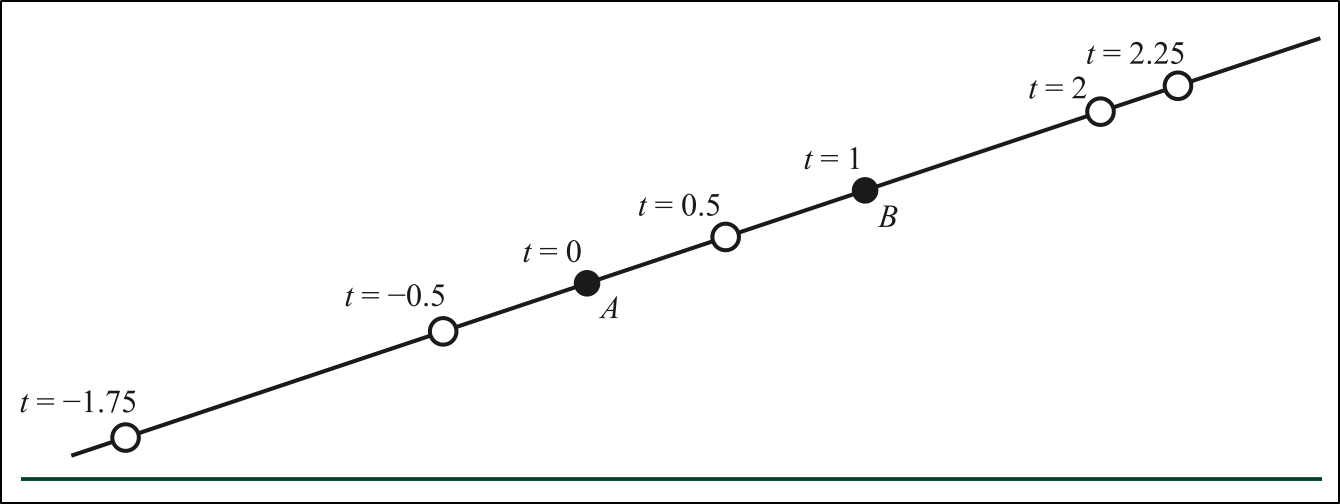
\includegraphics[width=0.8\textwidth]{parametric_line_gems}
    \caption[]{How changing values of t gives different points on the line.}
    \label{fig:parametric_line_gems}
\end{figure}

Instead of two points, choosing a point and a direction is better. We can define point \textbf{$B$} as \textbf{$d$} (\textit{direction}) and point \textbf{$A$} as \textbf{$O$} (\textit{origin}). For various computation reasons, like computing cosines with dot products, it's preferable to use a normalized vector as a direction:

\begin{equation}
    P(t) = O + t \hat{d}
\end{equation}

We may select any values of $t$ and the point $P$ moves continuously along the line. When we use a normalized vector as a direction, the value of $t$ represents the signed distance from the origin.

\begin{figure}[H]
    \centering
    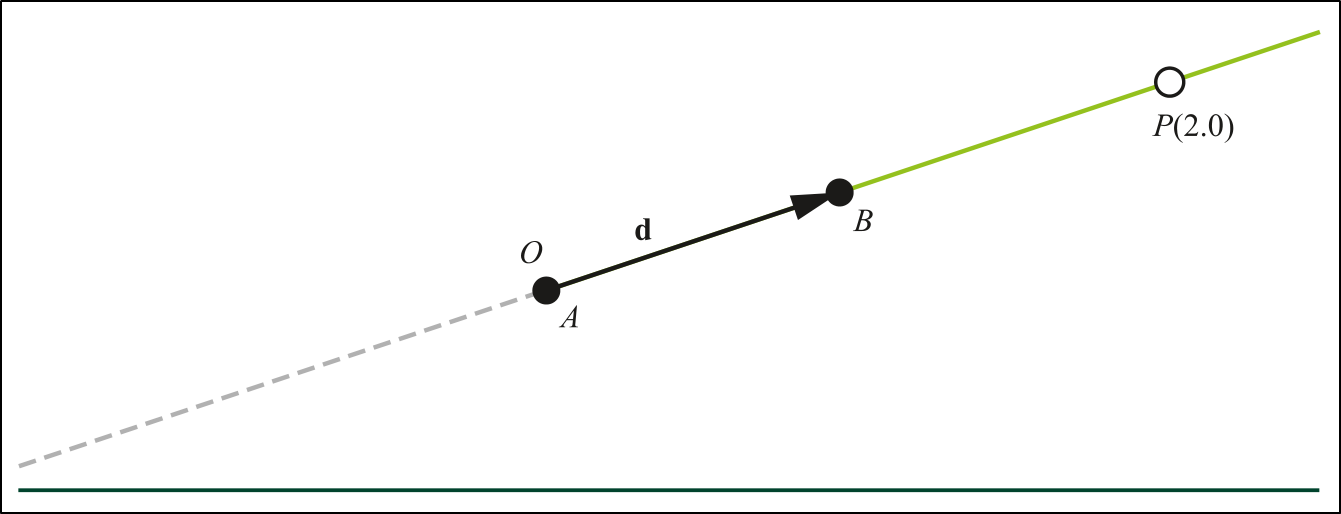
\includegraphics[width=0.8\textwidth]{ray_gems}
    \caption[]{A Ray, described by an origin $O$ and direction vector $\hat{d}$. The points are in front of the origins, i.e. $t > 0$. The dashed line represents points behind the origin.}
    \label{fig:ray_gems}
\end{figure}

\section{Intersections}

Once we generate a ray, we need to wind its intersections with various geometrical objects. Different geometries can behave differently depending on the shape or material of an object. Historically, each ray training engine starts with ray-sphere interactions \cite{Haines_1989}:

\begin{figure}[H]
    \centering
    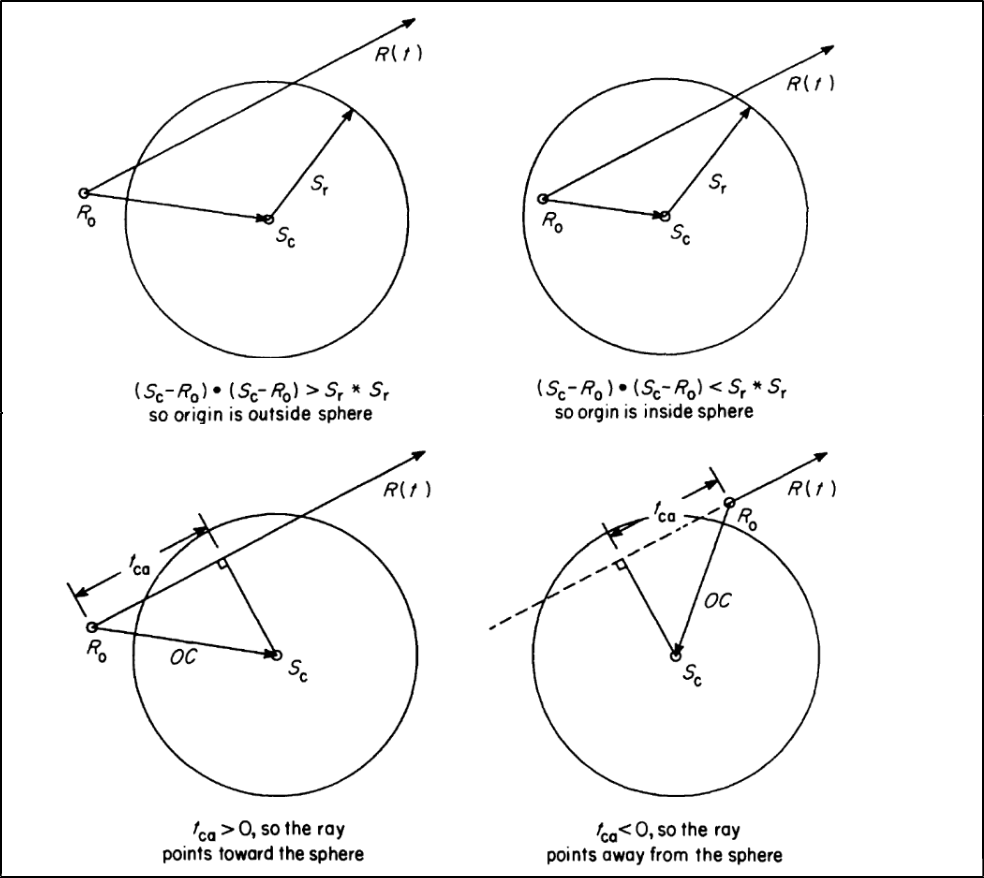
\includegraphics[width=0.8\textwidth]{ray-sphere-haines-89}
    \caption[]{The ray origin with respect to sphere location.}
    \label{fig:ray-sphere-haines-89}
\end{figure}

After defining intersections with spherical geometries, the ray tracing engine should get ray-plane intersections for constructing quadrilaterals and further usage in ray-polygon intersection algorithms.

We know a point is on the surface of a plane if it satisfies the plane equation:

\begin{equation}
    \begin{split}
    Plane = Ax + Bx + Cz + D = 0 \\ where: A^2 + B^2 + C^2 = 1
    \end{split}
\end{equation}

If no point along the ray satisfies the plane equation, the ray and plane do not intersect \cite{Szauer_2017}:

\begin{figure}[H]
    \centering
    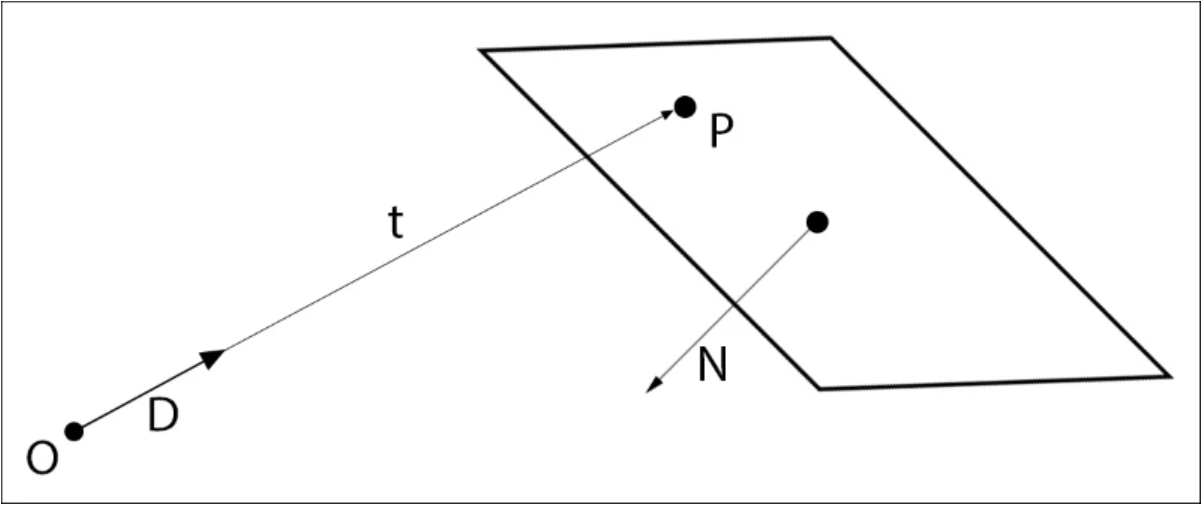
\includegraphics[width=0.8\textwidth]{ray-plane-intersection}
    \caption[]{Ray-Plane intersection diagram.}
    \label{fig:ray-plane-intersection}
\end{figure}

Once the ray-plane intersection is defined, the ray-polygon intersection can be performed. Eric Haines presented \cite{Haines_1989} one of many methods for testing the location of points (inside or outside), known as the Jordan curve theorem:

\begin{figure}[H]
    \centering
    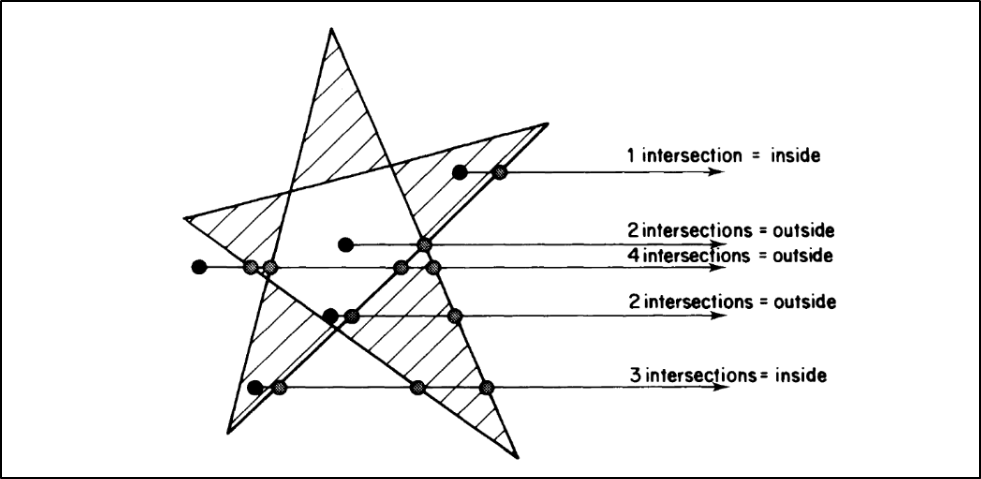
\includegraphics[width=0.8\textwidth]{jordan-curve-haines}
    \caption[]{Ray-Plane intersection diagram.}
    \label{fig:jordan-curve-haines}
\end{figure}

This algorithm works by shooting rays in an arbitrary direction and counting the number of intersections with the polygon. If the number is odd, the point is inside the polygon; otherwise, it is outside. The Jordan curve theorem is a fundamental concept in computational geometry. Once the ray-polygon interacting achieved, the ray tracing engine can construct more complex geometries like triangles quadrilaterals, and other polygons.

\newpage
\section{Optimization}

Another important area in ray tracing is performance optimizations and acceleration techniques. Using different geometry structures allows for the reduction of complicated computations, increasing the rendering time of a scene. The figure \ref{fig:acceleration-techniques} presents the broad classification of various optimization approaches described by Arvo and Kirk \cite{Arvo_Kirk_1989}.

\begin{figure}[H]
    \centering
    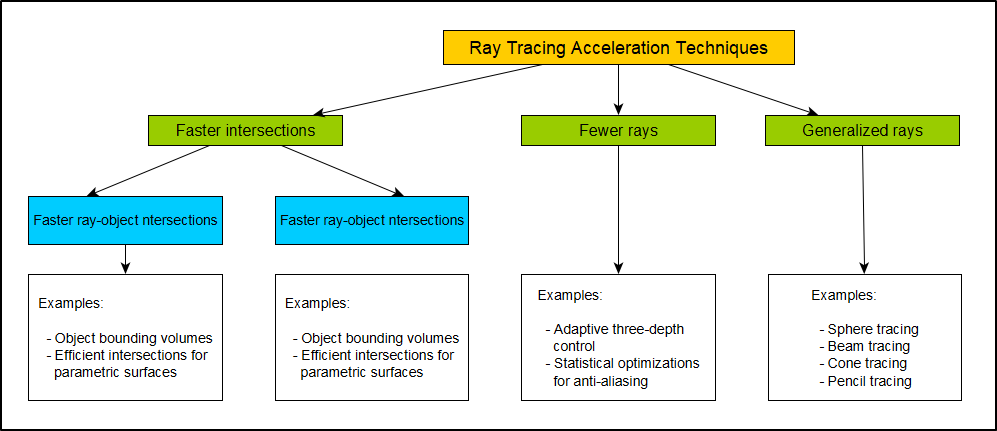
\includegraphics[width=0.8\textwidth]{acceleration-techniques}
    \caption[]{A broad classification of acceleration techniques.}
    \label{fig:acceleration-techniques}
\end{figure}

BVH trees are the most important optimization technology in ray tracing. A scene can consist of thousands of objects. Some of them are visible, some of them are not. If an object invisible, it could be traceable or not traceable. BVH constructions and bounding box hit-checking algorithms help to the time of initial scene construction and ray-tracing computations. The figures \ref{fig:bvh-100}, \ref{fig:bvh-1000}, \ref{fig:bvh-5000}, \ref{fig:bvh-10000}, \ref{fig:bvh-20000} show the increasing number of objects on the ray traced scene. Each of the spheres wrapped into a bounding box and the whole scene exists as one BVH construction.

\begin{multicols}{5}
    \begin{figure}[H]
        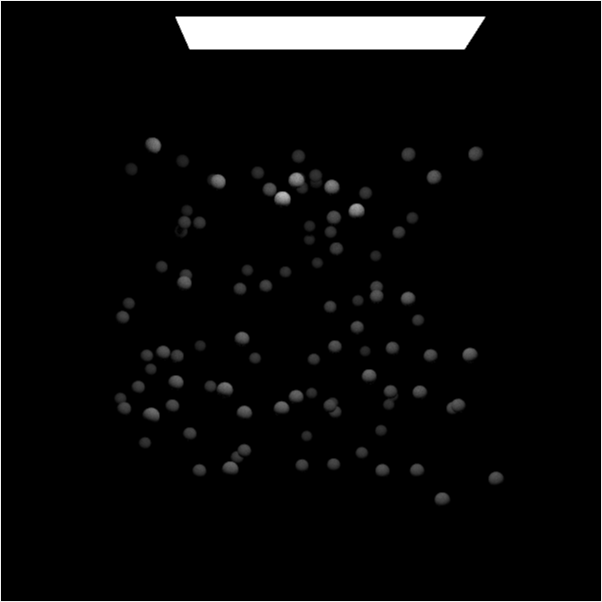
\includegraphics[width=0.18\textwidth]{bvh-100}
        \caption[]{\\100 objects\\Time: 5s}
        \label{fig:bvh-100}
    \end{figure}
    \columnbreak
    \begin{figure}[H]
        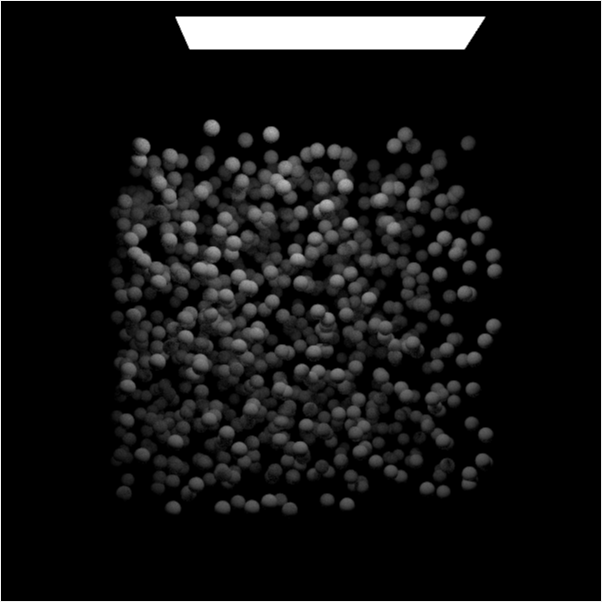
\includegraphics[width=0.18\textwidth]{bvh-1000}
        \caption[]{\\1000 objects\\Time: 27s}
        \label{fig:bvh-1000}
    \end{figure}
    \columnbreak
    \begin{figure}[H]
        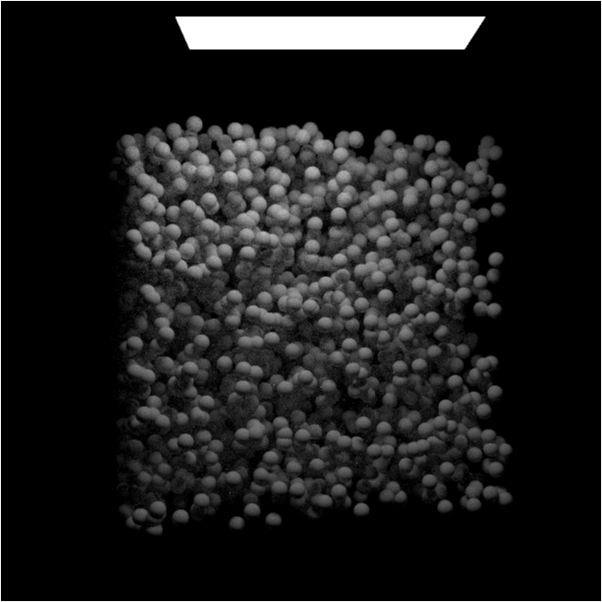
\includegraphics[width=0.18\textwidth]{bvh-5000}
        \caption[]{\\5000 objects\\Time: 106s}
        \label{fig:bvh-5000}
    \end{figure}
    \columnbreak
    \begin{figure}[H]
        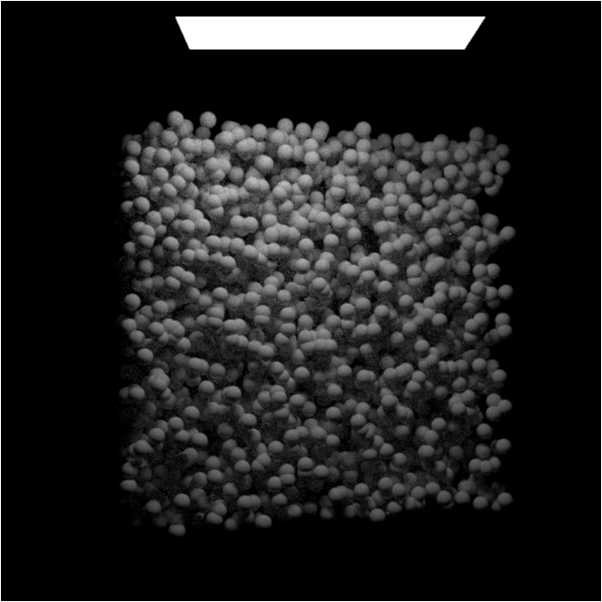
\includegraphics[width=0.18\textwidth]{bvh-10000}
        \caption[]{\\10000 objects\\Time: 112s}
        \label{fig:bvh-10000}
    \end{figure}
    \columnbreak
    \begin{figure}[H]
        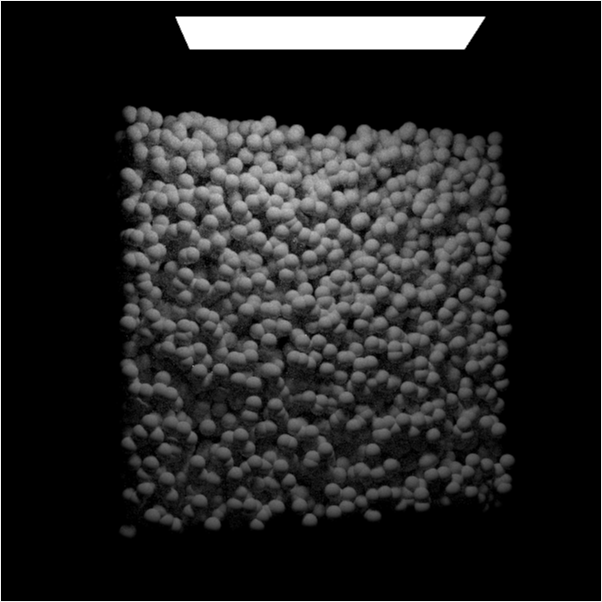
\includegraphics[width=0.18\textwidth]{bvh-20000}
        \caption[]{\\20000 objects\\Time: 149s}
        \label{fig:bvh-20000}
    \end{figure}
\end{multicols}

As was shown in the figures above, the computation time for 100 samples per pixel doesn't increase too much when sphered starting to overlap each other.

Another interesting optimization approach proposed by Alexander Reshetov \cite{Reshetov_2019}. Their GARP method (Geometric Approach to Ray/bilinear Patch intersections) is trying to find a balance between the simplicity of triangles and the richness of such smooth shapes as subdivision surfaces, NURBS, and Bézier patches.

The intersection point could be computed as either $X_r = R(t)$ or as $X_q = Q(u, v)$ using the found parameters $t$, $u$, and $v$. The two-step GARP process dynamically reduces a possible error in each step. In the first step, we find the best estimation for $u$. On the second step, using the found $u-aim$, minimizing the total error.

\begin{figure}[H]
    \centering
    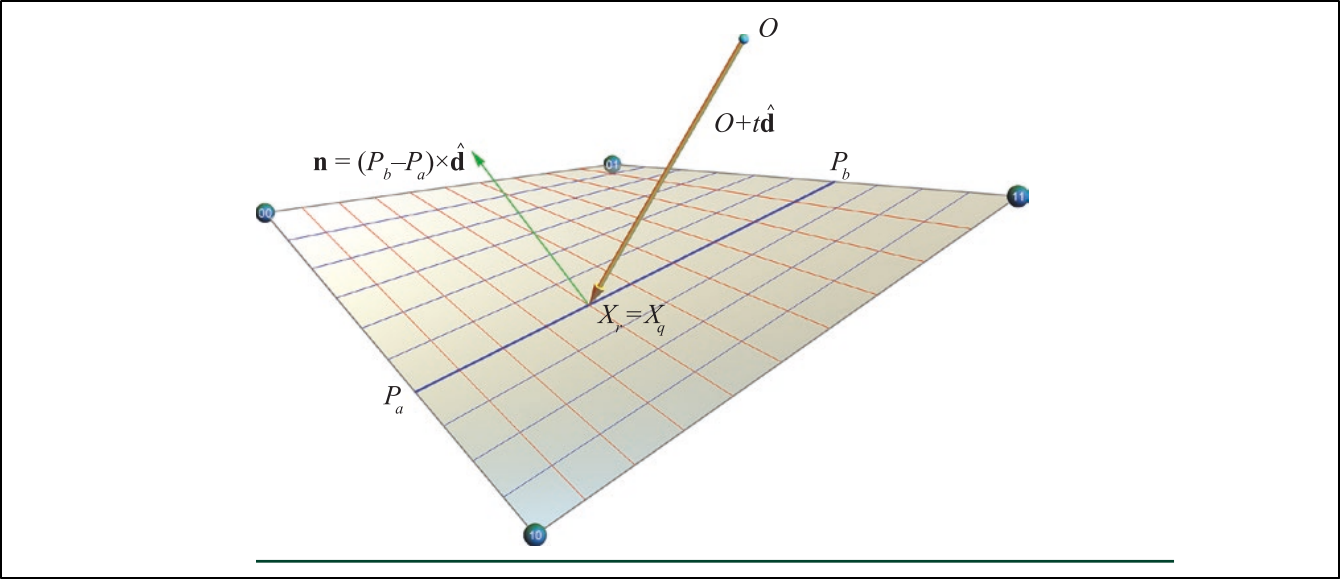
\includegraphics[width=0.8\textwidth]{garp}
    \caption[]{Finding ray/patch intersections.}
    \label{fig:garp}
\end{figure}

The figure \ref{fig:garp_bunny} shows the performance measurements performed by the author by counting the total number of rays processed per second.

\begin{figure}[H]
    \centering
    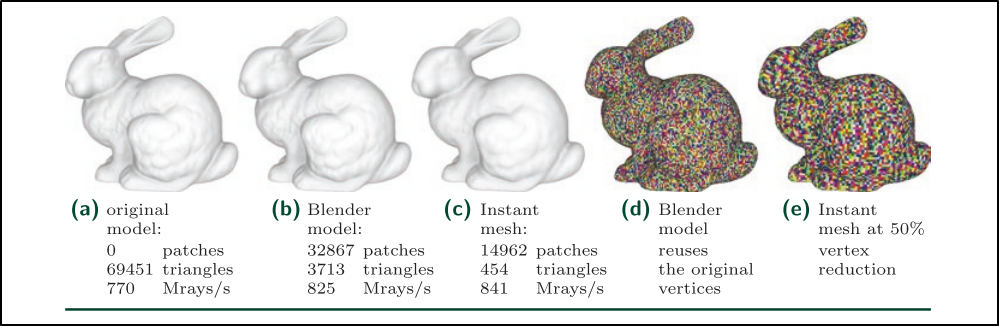
\includegraphics[width=0.8\textwidth]{garp_bunny}
    \caption[]{Finding ray/patch intersections.}
    \label{fig:garp_bunny}
\end{figure}

\section{Conclusion}

As was shown, the computational geometry is the essential part of the ray tracing ecosystem that works in different areas: scene construction, object relations, and optimizations.

\nocite{*}
\bibliographystyle{alpha}
\bibliography{common/references}

\end{document}
